\documentclass[slovene,11pt,a4paper]{article}
\usepackage[margin=2cm,bottom=3cm,foot=1.5cm]{geometry}

\setlength{\parindent}{0pt}
\setlength{\parskip}{0.5ex}

\usepackage[pdftex]{graphicx}
\DeclareGraphicsExtensions{.pdf,.png}


\usepackage{amsmath}
\usepackage{amsfonts}
\usepackage{mathrsfs}
\usepackage[usenames]{color}
\usepackage[slovene]{babel}
\usepackage[utf8]{inputenc}
\usepackage{siunitx}
\usepackage{subcaption}
\usepackage{float}

\def\phi{\varphi}
\def\eps{\varepsilon}
\def\theta{\vartheta}

\newcommand{\thisyear}{2025/26}

\renewcommand{\Re}{\mathop{\rm Re}\nolimits}
\renewcommand{\Im}{\mathop{\rm Im}\nolimits}
\newcommand{\Tr}{\mathop{\rm Tr}\nolimits}
\newcommand{\diag}{\mathop{\rm diag}\nolimits}
\newcommand{\dd}{\,\mathrm{d}}
\newcommand{\ddd}{\mathrm{d}}
\newcommand{\ii}{\mathrm{i}}
\newcommand{\lag}{\mathcal{L}\!}
\newcommand{\ham}{\mathcal{H}\!}
\newcommand{\four}[1]{\mathcal{F}\!\left(#1\right)}
\newcommand{\bigO}[1]{\mathcal{O}\!\left(#1\right)}
\newcommand{\sh}{\mathop{\rm sinh}\nolimits}
\newcommand{\ch}{\mathop{\rm cosh}\nolimits}
\renewcommand{\th}{\mathop{\rm tanh}\nolimits}
\newcommand{\erf}{\mathop{\rm erf}\nolimits}
\newcommand{\erfc}{\mathop{\rm erfc}\nolimits}
\newcommand{\sinc}{\mathop{\rm sinc}\nolimits}
\newcommand{\rect}{\mathop{\rm rect}\nolimits}
\newcommand{\ee}[1]{\cdot 10^{#1}}
\newcommand{\inv}[1]{\left(#1\right)^{-1}}
\newcommand{\invf}[1]{\frac{1}{#1}}
\newcommand{\sqr}[1]{\left(#1\right)^2}
\newcommand{\half}{\frac{1}{2}}
\newcommand{\thalf}{\tfrac{1}{2}}
\newcommand{\pd}{\partial}
\newcommand{\Dd}[3][{}]{\frac{\ddd^{#1} #2}{\ddd #3^{#1}}}
\newcommand{\Pd}[3][{}]{\frac{\pd^{#1} #2}{\pd #3^{#1}}}
\newcommand{\avg}[1]{\left\langle#1\right\rangle}
\newcommand{\norm}[1]{\left\Vert #1 \right\Vert}
\newcommand{\braket}[2]{\left\langle #1 \vert#2 \right\rangle}
\newcommand{\obraket}[3]{\left\langle #1 \vert #2 \vert #3 \right \rangle}
\newcommand{\hex}[1]{\texttt{0x#1}}

\renewcommand{\iint}{\mathop{\int\mkern-13mu\int}}
\renewcommand{\iiint}{\mathop{\int\mkern-13mu\int\mkern-13mu\int}}
\newcommand{\oiint}{\mathop{{\int\mkern-15mu\int}\mkern-21mu\raisebox{0.3ex}{$\bigcirc$}}}

\newcommand{\wunderbrace}[2]{\vphantom{#1}\smash{\underbrace{#1}_{#2}}}

\renewcommand{\vec}[1]{\overset{\smash{\hbox{\raise -0.42ex\hbox{$\scriptscriptstyle\rightharpoonup$}}}}{#1}}
\newcommand{\bec}[1]{\mathbf{#1}}



\title{
\sc\large Matematično-fizikalni praktikum \thisyear\\
\bigskip
\bf\Large 3.~naloga: Lastne vrednosti in lastni vektorji
}
\author{Samo Krejan, 28231092}
\date{}

\newcommand{\Ai}{\mathrm{Ai}}
\newcommand{\Bi}{\mathrm{Bi}}
\newcommand{\bi}[1]{\hbox{\boldmath{$#1$}}}
\newcommand{\bm}[1]{\hbox{\underline{$#1$}}}


\begin{document}
\maketitle
% \vspace{-1cm}

Enodimenzionalni linearni harmonski oscilator (delec mase $m$
s kinetično energijo $T(p)=p^2/2m$ v kvadratičnem potencialu
$V(q)=m\omega^2 q^2/2$) opišemo z brezdimenzijsko Hamiltonovo funkcijo
\begin{equation*}
  H_0 = {1\over 2} \left( p^2 + q^2 \right) \>,
\end{equation*}
tako da energijo merimo v enotah $\hbar\omega$, gibalne količine
v enotah $(\hbar m\omega)^{1/2}$ in dolžine v enotah $(\hbar/m\omega)^{1/2}$.
Lastna stanja $|n\rangle$ nemotenega Hamiltonovega operatorja $H_0$
poznamo iz osnovnega tečaja kvantne mehanike [Strnad III]:
v koordinatni reprezentaciji so lastne valovne funkcije
\begin{equation*}
  |n\rangle = (2^n n! \sqrt{\pi})^{-1/2} \mathrm{e}^{-q^2/2}\,  {\cal H}_n (q)\>,
\end{equation*}
kjer so ${\cal H}_n$ Hermitovi polinomi.
Lastne funkcije zadoščajo stacionarni Schr\"odingerjevi enačbi
\begin{equation*}
H_0 | n^0 \rangle = E_n^0 | n^0 \rangle
\end{equation*}
z nedegeneriranimi lastnimi energijami $E_n^0 = n + 1/2$
za $n=0,1,2,\ldots~$.  Matrika $\langle i | H_0 | j\rangle$
z $i,j=0,1,2,\ldots,N-1$ je očitno diagonalna, z vrednostmi
$\delta_{ij}(i + 1/2)$ po diagonali.  Nemoteni Hamiltonki
dodamo anharmonski člen
\begin{equation*}
H = H_0 + \lambda q^4 \>.
\end{equation*}
Kako se zaradi te motnje spremenijo lastne energije?
Iščemo torej matrične elemente $\langle i | H | j\rangle$
{\sl motenega\/} Hamiltonovega operatorja v bazi {\sl nemotenih\/}
valovnih funkcij $| n^0\rangle$, kar vemo iz perturbacijske
teorije v najnižjem redu.  Pri računu si pomagamo
s pričakovano vrednostjo prehodnega matričnega
elementa za posplošeno koordinato
$$
q_{ij} = \langle i | q | j \rangle
       = {1\over 2} \sqrt{i+j+1}\,\, \delta_{|i-j|,1} \>,
$$
ki, mimogrede, uteleša izbirno pravilo za električni dipolni
prehod med nivoji harmonskega oscilatorja.  V praktičnem računu
moramo seveda matriki $q_{ij}$ in $\langle i | H | j\rangle$
omejiti na neko končno razsežnost $N$.

\section{Naloga}

Z diagonalizacijo poišči nekaj najnižjih lastnih
vrednosti in lastnih valovnih funkcij za moteno Hamiltonko
$H = H_0 + \lambda q^4$
ob vrednostih parametra $0\le\lambda\le 1$.

\subsection{Sestavljanje Hamiltonke}

Namesto da računamo matrične elemente
$q_{ij}=\langle i | q | j \rangle$ in perturbacijsko matriko
razumemo kot $[ q_{ij} ]^4$, bi lahko računali tudi matrične
elemente kvadrata koordinate
\begin{equation*}
q^{(2)}_{ij} = \langle i | q^2 | j \rangle
\end{equation*}
in motnjo razumeli kot kvadrat ustrezne matrike,
\begin{equation*}
\lambda q^4 \to \lambda \left[ \, q^{(2)}_{ij} \,\right]^2 \>,
\end{equation*}
ali pa bi računali matrične elemente četrte potence koordinate
\begin{equation*}
q^{(4)}_{ij} = \langle i | q^4 | j \rangle
\end{equation*}
in kar to matriko razumeli kot motnjo,
\begin{equation*}
\lambda q^4 \to \lambda \left[ \, q^{(4)}_{ij} \,\right] \>.
\end{equation*}

Pri implementaciji slednjih načinov si lahko pomagamo z naslednjima formulama za povprečno vrednost matričnega elementa

\begin{equation*}
\langle i|q^2|j\rangle
  = {1\over 2} \biggl[
    {\sqrt{j(j-1)}} \, \delta_{i,j-2}
  + {(2j+1)} \, \delta_{i,j}
  + {\sqrt{(j+1)(j+2)}} \, \delta_{i,j+2} \biggr]
\end{equation*}
ter
\begin{eqnarray*}
\langle i|q^4|j\rangle
  = {1\over 2^4}\sqrt{2^i \, i!\over 2^{j} \, j! } \, \biggl[ \,
  &\,& \delta_{i,j+4} + 4\left(2j+3\right) \delta_{i,j+2}
                      + 12 \left(2j^2+2j+1\right) \, \delta_{i,j} \\[3pt]
  &+& 16j \left(2j^2-3j+1\right) \, \delta_{i,j-2}
     + 16j\left(j^3-6j^2+11j-6\right) \, \delta_{i,j-4} \biggr] \>,
\end{eqnarray*}
ki ju ni težko izpeljati iz rekurzijskih zvez za Hermitove
polinome.

\bigskip

Torej imamo tri pametne načine kako dobiti elemente Hamiltonke. Ti se seveda razlikujejo tako v natančnosti, kot pa tudi v času potrebnem za sestavo. Poglejmo si najprej kako je s časom, odvisnost potrebnega časa od velikosti matrike je za vse tri načine prikazana na grafu \ref{fig: q4 speed}

\begin{figure}[ht]
\begin{center}
  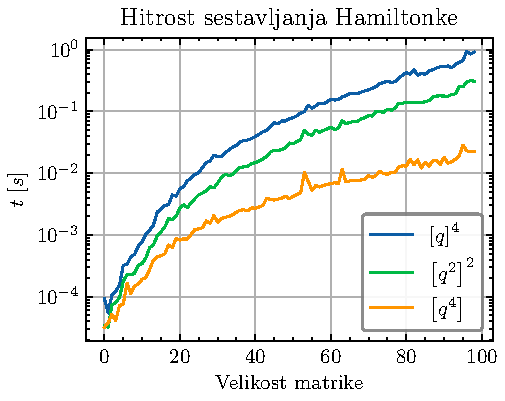
\includegraphics[width=10cm]{graphs/q4_speed.pdf}
  \caption{Odvisnost potrebnega časa za sestavljanje Hamiltonke v odvisnosti od njene velikosti}
  \label{fig: q4 speed}
\end{center}
\end{figure}

Vidimo da je daleč najhitrejša zadnja metoda. Seveda, vemo le da to velja le za našo implementacijo, ki verjetno ni optimalna. Namreč, matrike s katerimi imamo opravka imajo večino členov enakih 0, kar bi lahko upoštevali tako, da bi definirali redko matriko, a ker tega ne storimo je kvadriranje matrike časovno zelo zahtevna operacija. Kljub temu ostanemo pri uporabi načina, ki se ne zanaša na potenciranje matrike saj se s tem izognemo tudi robnim defektom, ki jih srečamo, ko potenciramo matriko, ki bi morala biti neskončna. Napako ki jo na ta način pridelamo z metodama $\left[q\right]^4$ in $\left[q^2\right]^2$ predstavimo na grafu \ref{fig: robni defekt} kjer dobimo zelo dober občutek za dogajanje na robu matrike:
\newpage
\begin{figure}[ht]
  \centering
  \begin{minipage}{0.48\textwidth}
    \centering
    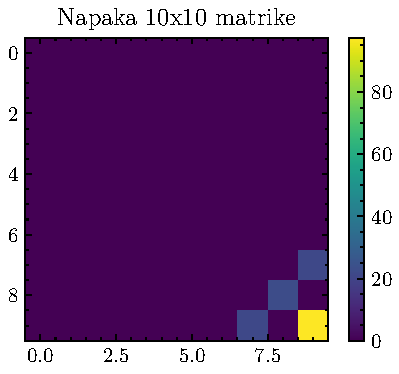
\includegraphics[width=\linewidth]{graphs/err1.pdf}
    
  \end{minipage}%
  \hfill%
  \begin{minipage}{0.48\textwidth}
    \centering
    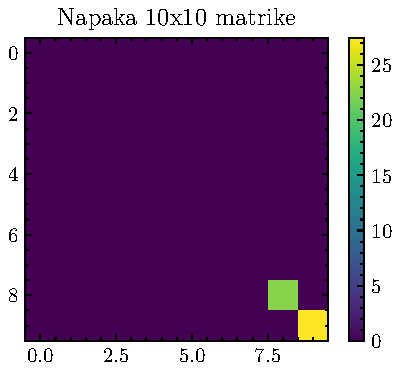
\includegraphics[width=\linewidth]{graphs/err2.pdf}
    
  \end{minipage}
  \caption{Na levi je prikazana napaka matrike sestavljene kot $\left[q\right]^4$ na desni pa kot $\left[q^2\right]^2$. Obe sta prikazani v obliki t.i. \textit{heatmapa}, kjer barva predstavlja vrednost v vsaki celici. Vidimo, da do napak pride res zgolj na robovim matrike.}
  \label{fig: robni defekt}
\end{figure}

Vidimo, da je res precej lažje le ne skrbeti in uporabiti $\left[q^4\right]$ način. To nato le pomnožimo z $\lambda$ in prištejemo $H_0$ in dobimo našo Hamiltonko.
\bigskip
\bigskip
\bigskip

\subsection{Računanje lastnih vrednosti}

Če želimo rešiti stacionarno Schr\"odingerjevo enačbo moramo poiskati lastne vrednosti in lastne vektorje Hamiltonke, sepravi nekakšne matrike. Za ta namen obstaja več različnih algoritmov, med drugimi tudi: QR iteracija, Jacobijev algoritem in Lanzcosov algoritem, ki sem jih implementiral na roke v programskem jeziku $Rust$, ki je mnogo hitrejši od $Python$ programskega jezika. Na tej točki moram priznati, da je veliko dela zame naredil ChatGPT. Sam sem se namreč šele učil Rust jezika, tako da sem ChatGPT prosil če mi napiše tri omenjene algoritme, kar pa mu je uspelo še preveč dobro. Večino mojega dela je bilo tako le  preverjati, da je vse implementirano pravilno, kjer sem moral narediti le manjše popravke. Opazil sem tudi, da bi lahko spet pri vseh algoritmih upošteval da gre za $redke$ matrike in tako verjetno mnogo izboljšal učinkovitost kode. Izkazalo se je, da to ni zares potrebno, saj je Rust dovolj hiter, da tudi matrike velikosti 2000 x 2000 ne vzamejo preveč časa. 

Ostane nam torej primerjava predvsem med hitrostmi različnih algoritmov in pa v $numpy$ vgrajeno knjižnico za diagonalizacijo hermitskih matrik. Primerjava je vidna na sliki \ref{fig: algos}.

\begin{figure}[ht]
\begin{center}
  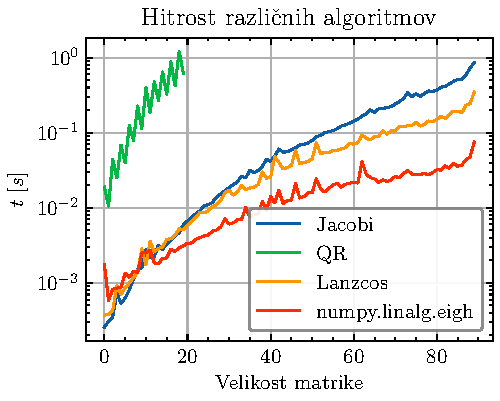
\includegraphics[width=10cm]{graphs/algos.pdf}
  \caption{Čas potreben za diagonalizacijo Hamiltonke v odvisnosti od velikosti le te.}
  \label{fig: algos}
\end{center}
\end{figure}

\newpage
Vidimo, da razen za nekaj malih vrednosti Numpy krepko premaga kateregakoli izmed mojih algoritmov. Še najbolje se odreže Lanzcosov algoritem, tako da sem se zanj odločil preveriti tudi natančnost, tako da sem za vsak par lastne vrednosti in pripadajočega lastnega vektorja ($\lambda_i$, $v_i$), matrike $H$; izračunal: $|Hv_i - \lambda_iv_i|_2$, ki nekako ustreza absolutni napaki naše diagonalizacije. Na ta način je nastal graf \ref{fig: err lanz}

\begin{figure}[ht]
  \centering
  \begin{minipage}{0.48\textwidth}
    \centering
    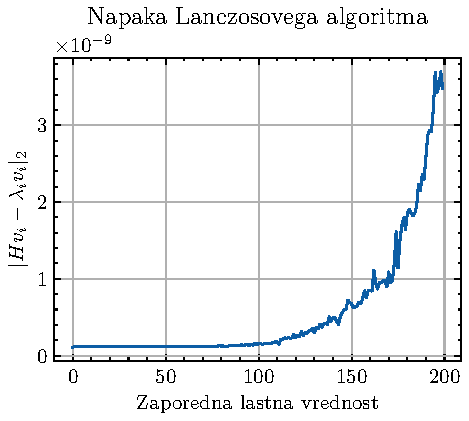
\includegraphics[width=\linewidth]{graphs/errlanz.pdf}
    
  \end{minipage}%
  \hfill%
  \begin{minipage}{0.48\textwidth}
    \centering
    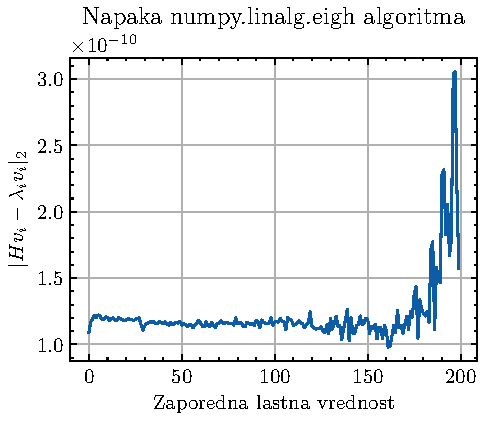
\includegraphics[width=\linewidth]{graphs/errnumpy.pdf}
    
  \end{minipage}
  \caption{Na levi je prikazana napaka prvih dvesto lastnih vrednosti in vektorjev izračunanih kot $|Hv_i - \lambda_iv_i|_2$ za mojo implementacijo Lanczosovega algoritma in na desni enako za numpy.linalg.eigh algoritem.}
  \label{fig: err lanz}
\end{figure}

Vidimo, da smo lahko precej zadovoljni z natančnostjo našega najuspešnejšega algoritma, čeprav je numpyjeva implementacija desetkrat natančnejša in hitrejša. Kljub dejstvu, da mi je lastna implementacija všeč, sem od te točke dalje uporabljal zgolj še numpy.linalg.eigh.

\newpage

\subsection{Lastne energije}

Poglaviten del naloge je iskanje lastnih energij motene Hamiltonke. Zanima nas kako so le te odvisne od parametra $\lambda$. A predno samo slepo računamo lastne vrednosti Hamiltonke in jih enačimo z lastnimi energijami se moramo vprašati, kako veliko matriko potrebujemo, da izračunamo določeno lastno energijo. Seveda lahko samo preprosto pretiravamo in vzamemo veliko preveliko matriko, recimo 2000 x 2000 in z njo poiščemo prvih 100 lastnih vrednosti, lahko pa analiziramo, ali lastne vrednosti Hamiltonke konvergirajo ko le to večamo. Prav te dve stvari lahko opazujemo na grafu \ref{fig: energ}.

\begin{figure}[ht]
  \centering
  \begin{minipage}{0.48\textwidth}
    \centering
    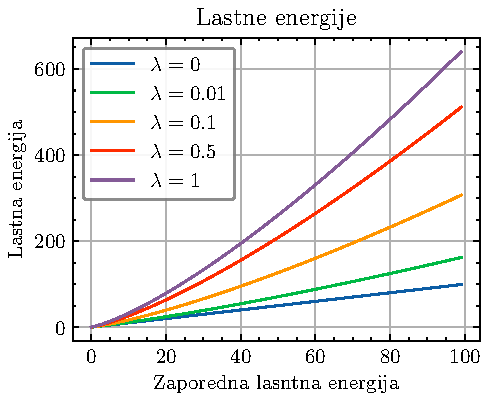
\includegraphics[width=\linewidth]{graphs/energ_.pdf}
    
  \end{minipage}%
  \hfill%
  \begin{minipage}{0.48\textwidth}
    \centering
    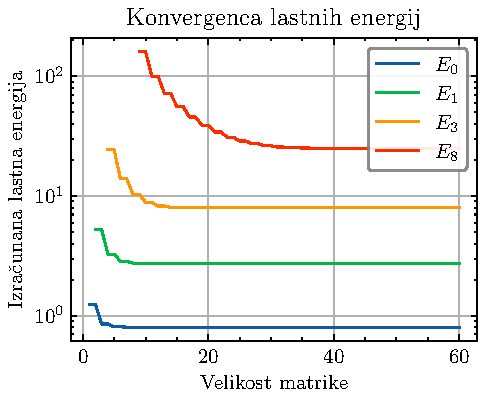
\includegraphics[width=\linewidth]{graphs/energ_konv.pdf}
    
  \end{minipage}
  \caption{Na levi strani vidimo, kako se lastne energije večajo z redom vzbuditve, na desni pa vidimo, kako vrednost lastnih energij konvergira z večanjem velikosti Hamiltonke (narisano za primer $\lambda = 0.5$)}
  \label{fig: energ}
\end{figure}

Iz grafa konvergence vidimo, da je potrebna vedno večja Hamiltonka, preden se lastna vrednost ustali. Smiselno se je vprašati, kako velika matrika je dejansko potrebna za določeno lastno vrednost, če želimo konstantno absolutno napako manjšo od recimo $10^{-6}$. Za oceno napake seveda potrebujemo 'pravo' vrednost posamezne lastne energije, za katero sem vzel preprosto lastne vrednosti izračunane iz matrike z velikostjo 3000. Potrebno velikost Hamiltonke za določene vrednosti parametra $\lambda$ smo nato poiskali z bisekcijo, in rezultate prikazali na grafu \ref{fig: dino}

\begin{figure}[ht]
\begin{center}
  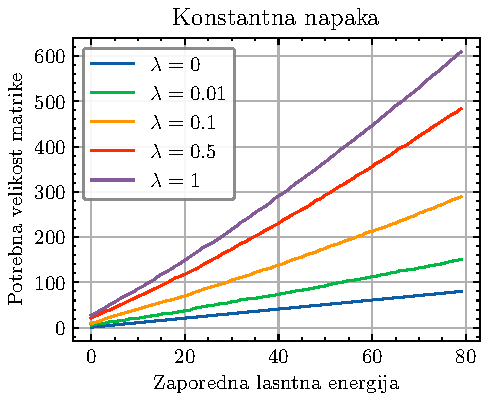
\includegraphics[width=8cm]{graphs/nodi.pdf}
  \caption{Potrebna velikost Hamiltonke za izračun lastne energije posameznega vzbujenega stanja}
  \label{fig: dino}
\end{center}
\end{figure}

Iz dobljenih grafov bi lahko ekstraporilali kako veliko matriko potrebujemo za natančen izračun tudi mnogo višjih vzbujenih stanj, a ko se približamo potrebni velikosti 3000, naša metoda seveda postane neuporabna.


\bigskip
\bigskip

\subsection{Lastne funkcije}

Ko smo računali lastne energije smo pravzaprav vedno zraven računali tudi lastne funkcije Hamiltonke. Pravzaprav smo računali lastne vektorje matrike Hamiltonke, kar pa je pravzaprav zgolj razvoj lastne funkcije po lastnih funkcijah harmonskega oscilatorja, ki je opisan v uvodu. Torej lastne funkcije izračunamo kot linearno kombinacijo lastnih funkcij harmonskega oscilatorja. Prve štiri lastne funkcije za različne $\lambda$ lahko prikažemo kar na istih oseh, da vidimo kako se funkcije spreminjajo z $\lambda$. To prikažemo na grafu \ref{fig: eig}.

\begin{figure}[ht]
  \centering
  \begin{minipage}{0.48\textwidth}
    \centering
    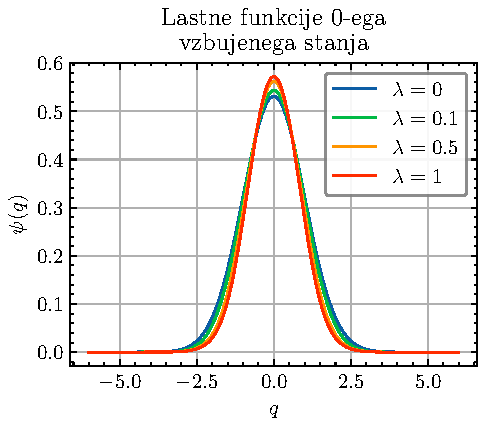
\includegraphics[width=\linewidth]{graphs/eig0.pdf}
    
  \end{minipage}%
  \hfill%
  \begin{minipage}{0.48\textwidth}
    \centering
    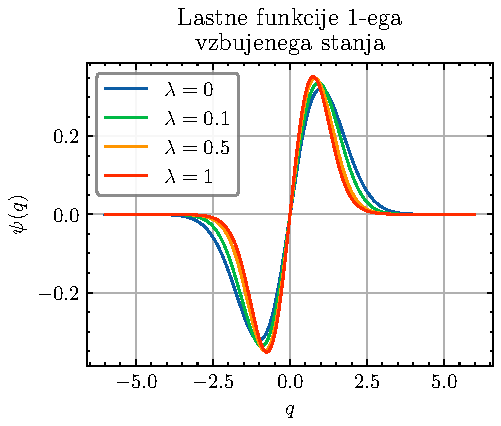
\includegraphics[width=\linewidth]{graphs/eig1.pdf}
    
  \end{minipage}

  \begin{minipage}{0.48\textwidth}
    \centering
    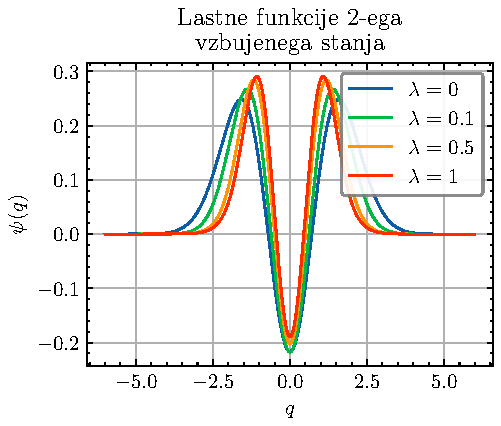
\includegraphics[width=\linewidth]{graphs/eig2.pdf}
    
  \end{minipage}%
  \hfill%
  \begin{minipage}{0.48\textwidth}
    \centering
    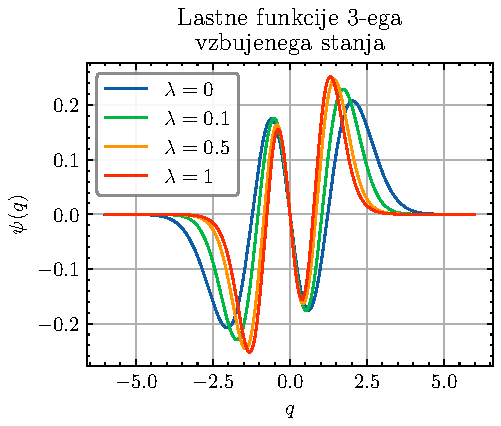
\includegraphics[width=\linewidth]{graphs/eig3.pdf}
    
  \end{minipage}
  \caption{Prve štiri lastne funkcije za različne vrednosti parametra $\lambda$}
  \label{fig: eig}
\end{figure}

Takoj opazimo nekaj lastnosti. Prva je ta, da so lastne funkcije ali sode ali lihe, kar je, kot smo se pri kvantni mehaniki naučili, posledica simetričnega potenciala. Za tem opazimo tudi, da ima večanje $\lambda$ nekakšen učinek \textit{stiskanja} lasnte funkcije, samo obliko pa le ta ohranja precej konstantno.

Lastne funkcije lahko narišemo še bolj intuitivno tako da jih narišemo na skupen graf, skupaj s skico potenciala, kjer vsako lastno funkcijo dvignemo za njeno lastno energijo. Točno to smo storili na grafu \ref{fig: pretty} za parameter $\lambda = 1$

\begin{figure}[ht]
\begin{center}
  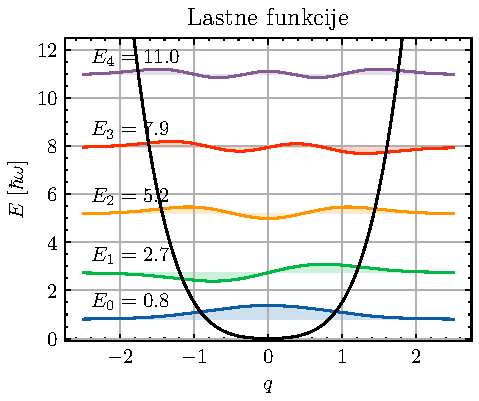
\includegraphics[width=10cm]{graphs/pretty.pdf}
  \caption{Lastne funkcije anharmonskega oscilatorja za $\lambda = 1$}
  \label{fig: pretty}
\end{center}
\end{figure}

Slednja reprezentacija se mi zdi zelo elegantna, saj jo je veliko lažje interpretirati kot pa vse različne črte na grafu \ref{fig: eig}

\section{Dodatna naloga}

\begin{quote}
  Poišči še nekaj najnižjih lastnih energij
in lastnih funkcij za problem v potencialu z dvema minimumoma
\begin{equation*}
H = {p^2\over 2} - 2q^2 + {q^4\over 10} \>.
\end{equation*}
\end{quote}

\subsection{Reševanje}

% 


\begin{figure}[ht]
  \centering
  \begin{minipage}{0.48\textwidth}
    \centering
    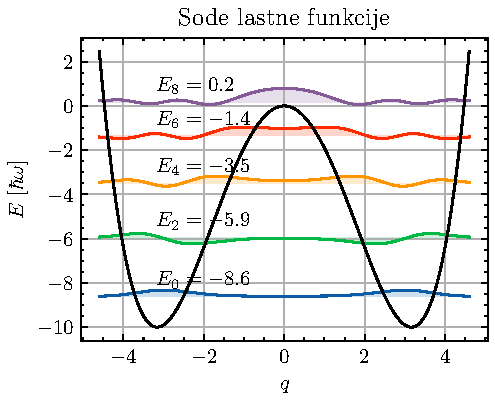
\includegraphics[width=\linewidth]{graphs/dodatnasod.pdf}
    
  \end{minipage}%
  \hfill%
  \begin{minipage}{0.48\textwidth}
    \centering
    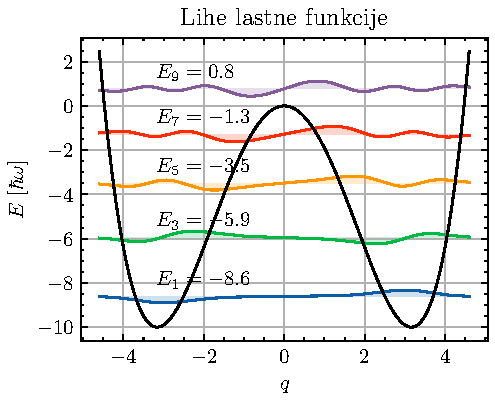
\includegraphics[width=\linewidth]{graphs/dodatnalih.pdf}
    
  \end{minipage}
  \caption{Sode in lihe lastne funkcije prikazane na ločenih grafih}
  \label{fig: dodatna}
\end{figure}

Samo reševanje problea se praktično nič ne razlikuje od tega, ki smo ga uporabljali do sedaj, tako da se lahko pravzaprav takoj osredotočimo na rezultat ki je prikazan na sliki \ref{fig: dodatna}. Prikaz lastnih funkcij smo razdelili na dva ločena grafa saj so zaporedne sode in lihe lastne energije skoraj enake. Pravzaprav bi skoraj lahko govorili o degeneriranih stanjih, a se izkaže da je tudi med osnovnim in prvim vzbujenim stanjem nekaj malega ($10^{-7}\hbar \omega$) razlike. To da so stanja, še posebaj tista blizu osnovnemu skoraj degenerirana je tudi intuitivno smiselno, saj se pri nizkih energijah delec očitno najverjetneje nahaja v enem izmed minimumov. Ker sta ta dva minimuma relativno daleč narazen je za samo energijo skoraj vseeno ali sta stanja v vsakem minimumu poravnana (soda funkcija) ali ravno obratna (liha funkcija).

\section{Zaključek}

Po končani nalogi se počutim, kot da bi lahko rešil Schr\"odingerjevo enačbo za skoraj vsak potencial. To mi da seveda misliti, da je bila naloga uspešno rešena.

Zelo sem zadovoljen, da sem se tekom reševanja odločil pomočiti prste v Rust programski jezik, v katerem sem iskreno precej užival. Poleg tega, sem se naučil marsikaj novega tudi glede algoritmov za diagonalizacijo matrik, ter o matričnem reševanju Schr\"odingerjevih enačb.

Tudi tokrat mi je uspelo pošteno namučiti računalnik, sploh takrat, ko sem ponesreči dodal eno ničlo ko sem definiral velikost Hamiltonke. Seveda to ni bil edini problem na katerega sem naletel. Ko sem se učil uvažati Rust funkcije v Python sem ponesreči skoraj uničil celotno Python okolje v katerem sem reševal nalogo. Ta, sicer mala, napaka me je stala nekaj dodatnih ur, ki bi jih veliko raje preživel ležeče v postelji.



% \newpage
% \bibliographystyle{plain}
% \bibliography{references}


\end{document}